\documentclass[a4paper,11pt]{amsart}

\usepackage{a4wide}
\usepackage{amsmath}
\usepackage{amssymb}
\usepackage{amsthm}
\usepackage[czech]{babel}
\usepackage{bookmark}
\usepackage{enumerate}
\usepackage[T1]{fontenc}
\usepackage{forest}
\usepackage{hyperref}
\usepackage[utf8]{inputenc}
\usepackage{lmodern}
\usepackage{multicol}
\usepackage{tikz}

\theoremstyle{definition}
    \newtheorem{problem}{Příklad}

% \theoremstyle{remark}
%     \newtheorem*{steps}{Postup řešení}

\theoremstyle{plain}
    \newtheorem*{solution}{Řešení}
    

\DeclareRobustCommand\proves{\mathrel{|}\joinrel\mkern-.5mu\mathrel{-}}
\DeclareMathOperator{\Conseq}{Csq}
\DeclareMathOperator{\M}{M}

% hide solutions
\newif\ifhidesolutions
    \hidesolutionstrue
    % \hidesolutionsfalse

\ifhidesolutions
    \usepackage{environ}
    \NewEnviron{hide}{}
    \let\solution\hide
    \let\endsolution\endhide
\fi








\begin{document}

\section*{NAIL062 V\&P Logika: 4. sada příkladů}
% po 4. přednášce



\subsection*{Výukové cíle:} Po absolvování cvičení student

    \begin{itemize}\setlength{\itemsep}{0pt}
        \item zná potřebné pojmy z tablo metody (položka, tablo, tablo důkaz/zamítnutí, dokončená/sporná větev, kanonický model), umí je formálně definovat, uvést příklady
        \item zná všechna atomická tabla, a umí vytvořit vhodná atomická tabla pro libovolnou logickou spojku
        \item umí sestrojit dokončené tablo pro danou položku z dané (i nekonečné) teorie
        \item umí popsat kanonický model pro danou dokončenou bezespornou větev tabla
        \item umí aplikovat tablo metodu k řešení daného problému (slovní úlohy, aj.)
        \item zná větu o kompaktnosti, umí ji aplikovat
    \end{itemize}
    

\section*{Příklady na cvičení}


\begin{problem}
    
    Aladin našel v jeskyni dvě truhly, A a B. Ví, že každá truhla obsahuje buď poklad, nebo smrtonosnou past.
    \begin{itemize}
    \item Na truhle A je nápis: {\it ``Alespoň jedna z těchto dvou truhel obsahuje poklad.''}
    \item Na truhle B je nápis: {\it ``V truhle A je smrtonosná past.''}
    \end{itemize}
    Aladin ví, že buď jsou oba nápisy pravdivé, nebo jsou oba lživé.
    \begin{enumerate}[(a)]
        \item Vyjádřete Aladinovy informace jako teorii $T$ nad vhodně zvolenou množinou výrokových proměnných $\mathbb P$. (Vysvětlete význam jednotlivých výrokových proměnných v $\mathbb P$.)
        \item Pokuste se sestrojit tablo důkazy, z teorie $T$, výroků o významu ``Poklad je v truhle A'' a ``Poklad je v truhle B''.
        \item Je-li některé z těchto dokončených tabel bezesporné, sestrojte kanonický model pro některou z jeho bezesporných větví.
        \item Jaký závěr z toho můžeme učinit?
    \end{enumerate}

    \begin{solution}
                    
    \end{solution}

\end{problem}


\begin{problem}

    Uvažme nekonečnou výrokovou teorii (a) $T=\{p_{i+1} \to p_i\mid i\in \mathbb{N}\}$ (b) $T=\{p_i \to p_{i+1}\mid i\in \mathbb{N}\}$. Pomocí tablo metody najděte všechny modely $T$. Je každý model $T$ kanonickým modelem pro některou z větví tohoto tabla? %(Můžete se pokusit sestrojit také \emph{systematické} tablo.)

    \begin{solution}
                    
    \end{solution}

\end{problem}


\begin{problem}

    Navrhněte vhodná atomická tabla pro logickou spojku $\oplus$ (XOR) a ukažte, že souhlasí-li model s kořenem vašich atomických tabel, souhlasí i s některou větví.

    \begin{solution}
                    
    \end{solution}
        
\end{problem}


\begin{problem}
    Pomocí věty o kompaktnosti ukažte, že každé spočetné částečné uspořádání lze rozšířit na úplné (lineární) uspořádání.
\end{problem}
        
        
\section*{Další příklady k procvičení}


\begin{problem}

    Adam, Barbora a Cyril jsou vyslýcháni, při výslechu bylo zjištěno následující:
    \begin{enumerate}[(i)]\it
        \item Alespoň jeden z vyslýchaných říká pravdu a alespoň jeden lže.
        \item Adam říká: \emph{``Barbora nebo Cyril lžou''}
        \item Barbora říká: \emph{``Cyril lže''}
        \item Cyril říká: \emph{``Adam nebo Barbora lžou''}
    \end{enumerate}
    \begin{enumerate}[(a)]
        \item Zapište tvrzení $(i)$ až $(iv)$ jako výroky $\varphi_1$ až $\varphi_4$ nad množinou prvovýroků $\mathbb{P}=\{a,b,c\}$, přičemž $a,b,c$ znamená (po řadě), že {\it ``Adam/Barbora/Cyril říká pravdu''}.
        \item Pomocí tablo metody dokažte, že z teorie $T = \{\varphi_1, \dots, \varphi_4\}$ plyne, že Adam říká pravdu.
        \item Je teorie $T$ ekvivalentní s teorií $T' = \{\varphi_2, \varphi_3, \varphi_4\}$? Zdůvodněte.    
    \end{enumerate}
    
\end{problem}
        

\begin{problem}

    Pomocí tablo metody dokažte, že následující výroky jsou tautologie:
    \begin{enumerate}[(a)]
        \item $(p\to (q \to q))$
        \item $p \leftrightarrow \neg \neg  p$
        \item $\neg (p \vee q) \leftrightarrow (\neg p \wedge \neg q)$
        \item $(p \to q) \leftrightarrow (\neg q \to \neg p)$    
    \end{enumerate}

\end{problem} 
   

\begin{problem}
    
    Pomocí tablo metody dokažte nebo najděte protipříklad ve formě \emph{kanonického} modelu pro bezespornou větev.
    \begin{enumerate}[(a)]
        \item $\{ \neg q,\ p \vee q\} \models p$
        \item $\{ q \to p,\ r \to q,\ (r \to p) \to s\} \models s$
        \item $\{ p \to r,\ p \vee q,\ \neg s \to \neg q\} \models r \to s$
    \end{enumerate}

\end{problem}


\begin{problem}

    Pomocí tablo metody určete všechny modely následujících teorií:
    \begin{enumerate}[(a)]
        \item $\{(\neg p \vee q) \to (\neg q \wedge r)\}$
        \item $\{\neg q \to (\neg p \vee q),\ \neg p \to q,\ r \to q\}$
        \item $\{ q \to p,\ r \to q,\ (r \to p) \to s\}$
    \end{enumerate}

\end{problem}


\begin{problem} 
    Navrhněte vhodná atomická tabla a ukažte, že souhlasí-li model s kořenem vašich atomických tabel, souhlasí i s některou větví:
    \begin{itemize}
        \item pro Peirceovu spojku $\downarrow$ (NOR),
        \item pro Shefferovu spojku $\uparrow$ (NAND),
        \item pro $\oplus$ (XOR),
        \item pro ternární operátor ``if p then q else r'' (IFTE).
    \end{itemize}  
    
\end{problem}


\begin{problem}

    \emph{Half-adder circuit} je logický obvod se dvěma vstupními bity (bit 1, bit 2) a dvěma výstupními bity (carry, sum) znázorněný v následujícím diagramu:
    \begin{center}
        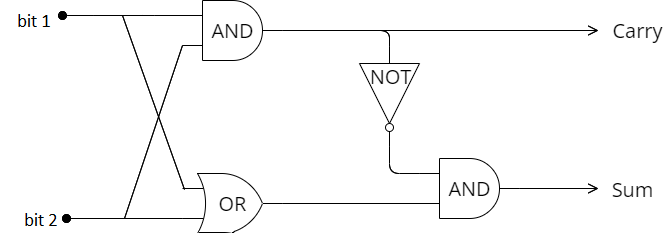
\includegraphics[width=0.5\textwidth]{files/half-adder.png}
    \end{center}
    \begin{enumerate}[(a)]
            \item Formalizujte tento obvod ve výrokové logice. Konkrétně, vyjádřete jej jako teorii $T=\{c\leftrightarrow \varphi,\ s\leftrightarrow \psi\}$ v jazyce $\mathbb P=\{b_1,b_2,c,s\}$, kde výrokové proměnné znamenají po řadě ``bit 1'', ``bit 2'', ``carry'' a ``sum'', a formule $\varphi,\psi$ neobsahují proměnné $c,s$.
            %\item Axiomatizujte teorii $T$ výrokem v CNF a také výrokem v DNF
            \item Dokažte tablo metodou, že $T\models c\to\neg s$.
            %\item Dokažte totéž rezoluční metodou (připomeňte si ji).
    \end{enumerate}

\end{problem}


\begin{problem}

    Pomocí věty o kompaktnosti dokažte, že každý spočetný rovinný graf je obarvitelný čtyřmi barvami. Můžete využít Větu o čtyřech barvách (pro konečné grafy).

\end{problem}

        
\section*{K zamyšlení}
        
        
\begin{problem}

    Dokažte přímo (transformací tabel) \emph{větu o dedukci}, tj. že pro každou teorii $T$ a výroky $\varphi$, $\psi$ platí:
    $$
    T \proves \varphi\to\psi\text{\ \ právě když\ \ }T,\varphi\proves  \psi
    $$

\end{problem}


\begin{problem}
    Mějme dvě neprázdné teorie $A, B$ v témž jazyce. Nechť platí, že každý model teorie $A$ splňuje alespoň jeden axiom teorie $B$. Ukažte, že existují konečné množiny axiomů $\{\alpha_1,\dots,\alpha_k\}\subseteq A$ a $\{\beta_1,\dots,\beta_n\}\subseteq B$ takové, že $\alpha_1\wedge\dots\wedge\alpha_k\,\to\,\beta_1\vee\dots\vee\beta_n$ je tautologie.
\end{problem}


\end{document}




